\documentclass[12pt]{article}
\usepackage[paper=letterpaper,margin=2cm]{geometry}
\usepackage{amsmath}
\usepackage{amssymb}
\usepackage{amsfonts}
\usepackage{newtxtext, newtxmath}
\usepackage{enumitem}
\usepackage{titling}
\usepackage{svg}
\usepackage{xcolor}
\usepackage{listings}
\usepackage{float}
\usepackage{nicefrac}
\usepackage{paracol}
\usepackage[most]{tcolorbox}
\usepackage[colorlinks=true]{hyperref}

\setlength{\droptitle}{-6em}

\definecolor{codegreen}{rgb}{0,0.6,0}
\definecolor{codegray}{rgb}{0.5,0.5,0.5}
\definecolor{codepurple}{rgb}{0.58,0,0.82}
\definecolor{backcolour}{rgb}{0.95,0.95,0.92}
\definecolor{bg}{rgb}{1,0.96,0.9}

\lstdefinestyle{mystyle}{
  commentstyle=\color{codegreen},
  keywordstyle=\color{magenta},
  numberstyle=\tiny\color{codegray},
  stringstyle=\color{codepurple},
  basicstyle=\ttfamily\footnotesize,
  breakatwhitespace=false,
  breaklines=true,
  captionpos=b,
  keepspaces=true,
  numbers=left,
  numbersep=5pt,
  showspaces=false,
  showstringspaces=false,
  showtabs=false,
  tabsize=2
}

\lstset{
  style=mystyle,
  inputencoding=utf8,
  extendedchars=true,
}


\begin{document}
\begin{enumerate}[leftmargin=\labelsep]
  \begin{tcolorbox}[enhanced jigsaw,halign=center,colback=bg,boxrule=0pt,arc=1pt]
    \item Consider the following unlabeled training data:
    \begin{table}[H]
      \centering
      \begin{tabular}{c|c|c}
              & $y_1$ & $y_2$ \\ \hline
        $x_1$ & 0     & 0     \\
        $x_2$ & 1     & 0     \\
        $x_3$ & 0     & 2     \\
        $x_4$ & 2     & 2
      \end{tabular}
    \end{table}

    Consider also the following initialization centroids:

    \begin{equation*}
      \mu_1 = \begin{bmatrix}
  80\\
  203.333\\
\end{bmatrix}, \quad \mu_2 = \begin{bmatrix}
  2\\
  1\\
\end{bmatrix}
    \end{equation*}

    \begin{enumerate}
      \item Apply $k$-means until convergence. What are the final centroids?
      \item Plot the data points and draw the clusters (with their respective centroids).
      \item Compute the silhouette score for sample $x_1$, cluster $c_1$ and for the overall solution.
      \item As the ground truth, take $x_3$ as a "negative" sample and the rest as "positive".
            Compute the error classification rate (ECR) of $k$-means here against the ground truth.
    \end{enumerate}
  \end{tcolorbox}

  For starters, it's probably worth it to write a general explanation of how $k$-means works.
  Basically, $k$-means is a clustering algorithm which, given a set of $n$ data points $\{x_1, \ldots, x_n\}$,
  tries to assign each data point to one of $k$ clusters. Each cluster is centered around
  a centroid $\mu_i$; while other clustering algorithms may create clusters of different shapes,
  $k$-means clusters are always circular/spherical. The algorithm works as follows:

  \begin{enumerate}
    \item Initialize the centroids $\mu_1, \ldots, \mu_n$.
    \item Assign each data point to the closest centroid.
    \item Recompute the centroids based on the assigned data points.
    \item Repeat steps b) and c) until convergence - that is, until the centroids don't change anymore
          (or until the change is below a certain threshold).
  \end{enumerate}

  In $k$-means solution implementations, we usually perform a series of runs with different
  centroid initializations and pick the best one (where the \textit{best} here
  is defined by a combination of metrics, which we'll discuss later). In the following
  exercises, though, we'll just use a single run. We'll also be using the Euclidian distance here,
  the most common distance metric used in this algorithm.

  For starters, let's assign each sample to the closest centroid. We can do this by computing
  the distance between each sample and each centroid, and then picking the centroid with the
  smallest distance:

  \begin{equation*}
    \left\| x_1 - \mu_1 \right\| = \left\| \begin{bmatrix}
  1 & 0 & 0 & 0\\
\end{bmatrix} - \begin{bmatrix}
  80\\
  203.333\\
\end{bmatrix} \right\|^2 = 4, \quad
    \left\| x_1 - \mu_2 \right\| = \left\| \begin{bmatrix}
  1 & 0 & 0 & 0\\
\end{bmatrix} - \begin{bmatrix}
  2\\
  1\\
\end{bmatrix} \right\|^2 = 5
  \end{equation*}

  $c = \operatorname{argmin}_{k \in \{1, 2\}} \left\| x_1 - \mu_n \right\|$ is, therefore, $k = 1$,
  and $x_1$ is assigned to cluster $c_1$.

  Performing similar computations for the other samples, we get the following:

  \begin{equation*}
    \begin{aligned}
      \operatorname{argmin}_{k \in \{1, 2\}} \left\| x_2 - \mu_n \right\| & = \operatorname{argmin}_{k \in \{1, 2\}} \{1, 2\} = c_1 \\
      \operatorname{argmin}_{k \in \{1, 2\}} \left\| x_3 - \mu_n \right\| & = \operatorname{argmin}_{k \in \{1, 2\}} \{8, 5\} = c_2 \\
      \operatorname{argmin}_{k \in \{1, 2\}} \left\| x_4 - \mu_n \right\| & = \operatorname{argmin}_{k \in \{1, 2\}} \{4, 1\} = c_2
    \end{aligned}
  \end{equation*}

  Now, we'll want to adjust our centroids: for each cluster, we'll compute the mean of all
  the samples assigned to it, and use that as the new centroid. $k$-means differs from
  other clustering algorithms here: EM, for example, utilizes every single sample in the
  dataset to compute the new centroids' parameters. $k$-means, on the other hand, by
  nature of working with hard assignments ends up using only a subset of the samples
  in the dataset to compute the new centroids.

  \begin{equation*}
    \mu_1 = \frac{1}{2} \left( x_1 + x_2 \right) = \frac{1}{2} \left( \begin{bmatrix}
  1 & 0 & 0 & 0\\
\end{bmatrix} + \begin{bmatrix}
  0\\
  1\\
\end{bmatrix} \right) = \begin{bmatrix}
  0.5\\
  0\\
\end{bmatrix}, \quad
    \mu_2 = \frac{1}{2} \left( x_3 + x_4 \right) = \frac{1}{2} \left( \begin{bmatrix}
  1 & 1 & 1 & 1\\
\end{bmatrix} + \begin{bmatrix}
  2\\
  2\\
\end{bmatrix} \right) = \begin{bmatrix}
  1\\
  2\\
\end{bmatrix}
  \end{equation*}

  The centroids have moved, so we'll have to repeat steps b) and c).

  \begin{equation*}
    \begin{aligned}
      \operatorname{argmin}_{k \in \{1, 2\}} \left\| x_1 - \mu_n \right\| & = \operatorname{argmin}_{k \in \{1, 2\}} \{0.25, 5\} = c_1 \\
      \operatorname{argmin}_{k \in \{1, 2\}} \left\| x_2 - \mu_n \right\| & = \operatorname{argmin}_{k \in \{1, 2\}} \{0.25, 4\} = c_1 \\
      \operatorname{argmin}_{k \in \{1, 2\}} \left\| x_3 - \mu_n \right\| & = \operatorname{argmin}_{k \in \{1, 2\}} \{4.25, 1\} = c_2 \\
      \operatorname{argmin}_{k \in \{1, 2\}} \left\| x_4 - \mu_n \right\| & = \operatorname{argmin}_{k \in \{1, 2\}} \{6.25, 1\} = c_2
    \end{aligned}
  \end{equation*}

  \begin{equation*}
    \mu_1 = \frac{1}{2} \left( x_1 + x_2 \right) = \frac{1}{2} \left( \begin{bmatrix}
  1 & 0 & 0 & 0\\
\end{bmatrix} + \begin{bmatrix}
  0\\
  1\\
\end{bmatrix} \right) = \begin{bmatrix}
  1.4\\
  1.2\\
  0.4\\
\end{bmatrix}, \quad
    \mu_2 = \frac{1}{2} \left( x_3 + x_4 \right) = \frac{1}{2} \left( \begin{bmatrix}
  1 & 1 & 1 & 1\\
\end{bmatrix} + \begin{bmatrix}
  2\\
  2\\
\end{bmatrix} \right) = \begin{bmatrix}
  1\\
  2\\
\end{bmatrix}
  \end{equation*}

  The centroids haven't moved, so we're done. At the end of the algorithm's run,
  the cluster assignments are as follows: $c_1 = \{x_1, x_2\}$, $c_2 = \{x_3, x_4\}$.

  Afterward, we can plot the clusters and the centroids (we can pretend that the
  cluster's circle is actually drawn and such), with $c_1$ in red and $c_2$ in blue:

  \begin{figure}[H]
    \centering
    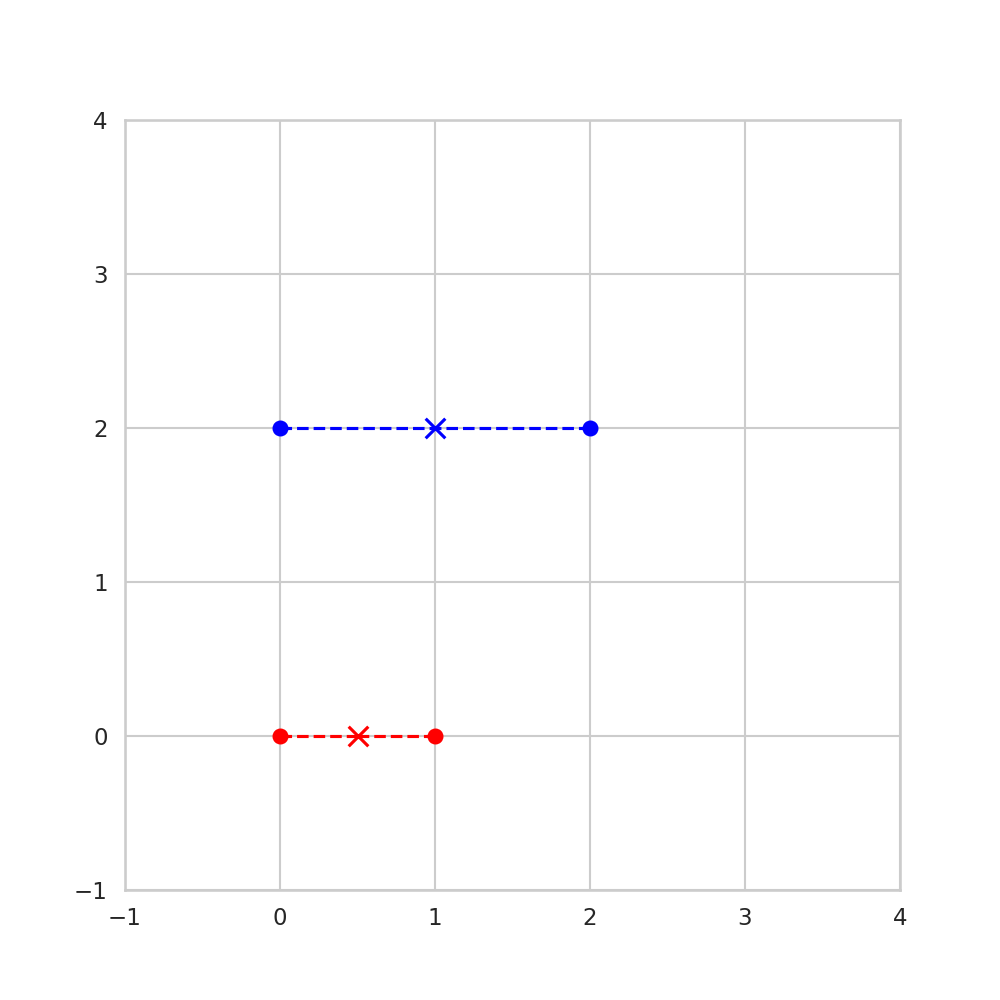
\includegraphics[width=0.43\textwidth]{assets/k-means-clusters.png}
    \label{fig:ex-1}
  \end{figure}

  Finally, regarding the \textbf{silhouette scores} of observations, we can compute them as follows
  (considering $s_n$ to be the silhouette of sample $x_n$ and $c_n$ to be its assigned cluster):

  \begin{equation*}
    \begin{aligned}
      s_n & = \frac{b_n - a_n}{\max\{a_n, b_n\}}                                                                            \\
      a_n & = \frac{1}{|c_n| - 1} \sum_{x_i \in c_n, x_i \neq x_n} \left\| x_i - x_n \right\|                               \\
      b_n & = \min_{n' \in \{1, \cdots, k\}, n' \neq n} \frac{1}{|c_{n'}|} \sum_{x_i \in c_{k'}} \left\| x_i - x_n \right\|
    \end{aligned}
  \end{equation*}

  Essentially, the silhouette score of a sample will take into account how close it is to
  the other samples in its cluster (in average), and how far it is from the samples in its
  most neighboring cluster (in average).

  \begin{equation*}
    \begin{aligned}
      a_1 & = \frac{1}{1} \left( \left\| x_2 - x_1 \right\| \right) =  1, \quad
      a_2 & = \frac{1}{1} \left( \left\| x_1 - x_2 \right\| \right) =  1        \\
      a_3 & = \frac{1}{1} \left( \left\| x_4 - x_3 \right\| \right) =  2, \quad
      a_4 & = \frac{1}{1} \left( \left\| x_3 - x_4 \right\| \right) = 2
    \end{aligned}
  \end{equation*}

  \begin{equation*}
    \begin{aligned}
      b_1 & = \min_{n' \in \{1, 2\}, n' \neq 1} \frac{1}{2} \left( \left\| x_3 - x_1 \right\| + \left\| x_4 - x_1 \right\| \right) = 2.414, \quad
      b_2 & = \min_{n' \in \{1, 2\}, n' \neq 1} \frac{1}{2} \left( \left\| x_3 - x_2 \right\| + \left\| x_4 - x_2 \right\| \right) = 2.236        \\
      b_3 & = \min_{n' \in \{1, 2\}, n' \neq 2} \frac{1}{2} \left( \left\| x_1 - x_3 \right\| + \left\| x_2 - x_3 \right\| \right) = 2.118, \quad
      b_4 & = \min_{n' \in \{1, 2\}, n' \neq 2} \frac{1}{2} \left( \left\| x_1 - x_4 \right\| + \left\| x_2 - x_4 \right\| \right) = 2.532
    \end{aligned}
  \end{equation*}

  \begin{equation*}
    \begin{aligned}
      s_1 & = \frac{2.414 - 1}{\max\{1, 2.414\}} = 0.5858, \quad
      s_2 & = \frac{2.236 - 1}{\max\{1, 2.236\}} = 0.5528        \\
      s_3 & = \frac{2.118 - 2}{\max\{2, 2.118\}} = 0.0557, \quad
      s_4 & = \frac{2.532 - 2}{\max\{2, 2.532\}} = 0.2102
    \end{aligned}
  \end{equation*}

  The silhouette scores for each cluster are given by the average of the silhouette
  scores of its samples:

  \begin{equation*}
    \begin{aligned}
      s_1 & = \frac{1}{2} \left( 0.5858 + 0.5528 \right) = 0.5693, \quad
      s_2 & = \frac{1}{2} \left( 0.0557 + 0.2102 \right) = 0.1329
    \end{aligned}
  \end{equation*}

  The overall silhouette score is given by the average of the silhouette scores of
  each cluster:

  \begin{equation*}
    s = \frac{1}{2} \left( 0.5693 + 0.1329 \right) = 0.3511
  \end{equation*}

  Finally, the \textbf{error classification rate} measures the proportion of misclassified
  samples in the dataset. If we think about the confusion matrix of the problem, we can
  write down the expression as:

  \begin{equation*}
    \begin{aligned}
      ECR & = \frac{FP + FN}{FP + FN + TP + TN} = \frac{1 + 1}{1 + 1 + 2 + 2} = 0.5
    \end{aligned}
  \end{equation*}

  \begin{tcolorbox}[enhanced jigsaw,halign=center,colback=bg,boxrule=0pt,arc=1pt]
    \item Consider the following unlabeled training data:

    \begin{table}[H]
      \centering
      \begin{tabular}{c|c|c|c}
              & $y_1$ & $y_2$ & $y_3$ \\ \hline
        $x_1$ & 1     & 0     & 0     \\
        $x_2$ & 8     & 8     & 4     \\
        $x_3$ & 3     & 3     & 0     \\
        $x_4$ & 0     & 0     & 1     \\
        $x_5$ & 0     & 1     & 0     \\
        $x_6$ & 3     & 2     & 1
      \end{tabular}
    \end{table}

    and let the initial $k$ centroids be the first $k$ samples.

    \begin{enumerate}
      \item Apply $k$-means until convergence, for $k \in \{2, 3\}$. What are the final centroids?
      \item Which $k$ provides a better clustering regarding \textbf{cohesion}
            (i.e the intra-cluster distance - the sum of the distances from every point to their centroid)?
      \item Which $k$ provides a better clustering regarding \textbf{separation}
            (i.e the inter-cluster distance - the average distance of every centroid to every other centroid)?
    \end{enumerate}
  \end{tcolorbox}

  Won't be doing the first question since it's basically repeating the last question's
  exercise (twice), and it's also in the teacher's solutions. We'll need the
  post-convergence centroids, though, so I'll write them down here (plus each
  cluster's assigned samples):

  \begin{paracol}{2}
    \setlength{\columnseprule}{1pt}
    \def\columnseprulecolor{\color{black}}
    \centering

    $k = 2$:

    \begin{equation*}
      \mu_1 = \begin{bmatrix}
  1.4\\
  1.2\\
  0.4\\
\end{bmatrix}, \quad \mu_2 = \begin{bmatrix}
  8\\
  8\\
  4\\
\end{bmatrix}
    \end{equation*}

    \begin{equation*}
      \begin{aligned}
        k_1 & = \{x_1, x_3, x_4, x_5, x_6\}, \quad
        k_2 & = \{x_2\}
      \end{aligned}
    \end{equation*}

    \switchcolumn

    $k = 3$:

    \begin{equation*}
      \mu_1 = \begin{bmatrix}
  0.333333\\
  0.333333\\
  0.333333\\
\end{bmatrix}, \quad \mu_2 = \begin{bmatrix}
  8\\
  8\\
  4\\
\end{bmatrix}, \quad \mu_3 = \begin{bmatrix}
  3\\
  2.5\\
  0.5\\
\end{bmatrix}
    \end{equation*}

    \begin{equation*}
      \begin{aligned}
        k_1 & = \{x_1, x_4, x_5\}, \quad
        k_2 & = \{x_2\}, \quad
        k_3 & = \{x_3, x_6\}
      \end{aligned}
    \end{equation*}

  \end{paracol}

  Regarding \textbf{cohesion}, we measure it as the sum of the distances from every
  point to their centroid. We can write down the expression as:

  \begin{equation*}
    \text{Cohesion}(k) = \sum_{i = 1}^k \sum_{x \in k_i} \left\| x - \mu_i \right\|^2
  \end{equation*}

  \begin{equation*}
    \begin{aligned}
      \text{Cohesion}(2) & = \left\| x_1 - \mu_1 \right\|^2 + \left\| x_2 - \mu_2 \right\|^2 + \left\| x_3 - \mu_1 \right\|^2 + \left\| x_4 - \mu_1 \right\|^2 + \left\| x_5 - \mu_1 \right\|^2 + \left\| x_6 - \mu_1 \right\|^2
                         &                                                                                                                                                                                                       & \approx 17.2 \\
      \text{Cohesion}(3) & = \left\| x_1 - \mu_1 \right\|^2 + \left\| x_2 - \mu_2 \right\|^2 + \left\| x_3 - \mu_3 \right\|^2 + \left\| x_4 - \mu_1 \right\|^2 + \left\| x_5 - \mu_1 \right\|^2 + \left\| x_6 - \mu_3 \right\|^2
                         &                                                                                                                                                                                                       & \approx 3.0
    \end{aligned}
  \end{equation*}

  Our goal is, ideally, to minimize this cohesion value: the closer the points are to
  their centroids, the better the clustering. We can see that $k = 3$ provides a
  better clustering in this regard, as expected: if there are more clusters, the
  points (generally speaking) should be able to better fit into them.

  \textbf{Separation}, on the other hand, is the average distance of every centroid to
  every other centroid. We can write down the expression as:

  \begin{equation*}
    \text{Separation}(k) = \frac{1}{k^2} \sum_{i = 1}^k \sum_{j = 1}^k \left\| \mu_i - \mu_j \right\|^2
  \end{equation*}

  \begin{equation*}
    \begin{aligned}
      \text{Separation}(2) & = \frac{1}{4} (\left\| \mu_1 - \mu_1 \right\|^2 + \left\| \mu_1 - \mu_2 \right\|^2 + \left\| \mu_2 - \mu_1 \right\|^2 + \left\| \mu_2 - \mu_2 \right\|^2)
      = \frac{1}{2} \left\| \mu_1 - \mu_2 \right\|^2
      \approx 51.38                                                                                                                                                                           \\
      \text{Separation}(3) & = \frac{1}{9} (\left\| \mu_1 - \mu_1 \right\|^2 + \left\| \mu_1 - \mu_2 \right\|^2 + \cdots \left\| \mu_3 - \mu_2 \right\|^2 + \left\| \mu_3 - \mu_3 \right\|^2)
      \approx 46.74
    \end{aligned}
  \end{equation*}

  As we've seen above, our previous goal was to minimize the cohesion value (for a
  better clustering solution); intuitively, we can say that growing separation values
  should lead to a better clustering solution, as well: the more separated the
  centroids are, (ideally) the better the clustering. We can see that $k = 3$ provides
  a worse clustering solution in this regard: the centroids are closer to each other,
  which means that the points could be more likely to be assigned to the wrong cluster.

  In the end, choosing the best $k$ value is a matter of balancing these (and other)
  metrics.

  \begin{tcolorbox}[enhanced jigsaw,halign=center,colback=bg,boxrule=0pt,arc=1pt]
    \item Consider the following data points:

    \begin{equation*}
      x_1 = (4), \quad x_2 = (0), \quad x_3 = (1)
    \end{equation*}

    Moreover, consider a mixture of two normal distributions with the following
    initialization of likelihoods and priors:

    \begin{equation*}
      \begin{aligned}
        \pi_1 & = P(c = k_1) = 0.5, \quad
              &                           & P(x | c = k_1) = \mathcal{N}(x; \mu_1, \sigma_1^2) = \mathcal{N}(x; 1, 1) \\
        \pi_2 & = P(c = k_2) = 0.5, \quad
              &                           & P(x | c = k_2) = \mathcal{N}(x; \mu_2, \sigma_2^2) = \mathcal{N}(x; 0, 1)
      \end{aligned}
    \end{equation*}

    Plot the clusters after a single iteration of the EM algorithm.

  \end{tcolorbox}

  The Expectation-Maximization (EM) algorithm is a powerful tool for cluster creation,
  learning the parameters of a distribution/mixture of distributions. It is a two-step iterative algorithm that
  alternates between two steps: the \textbf{Expectation} step and the
  \textbf{Maximization} step.

  Here, our centroids are precisely the means of each distribution; if in
  $k$-means we directly assigned the points to a cluster (and centroid updates
  would only take into account the samples assigned to them), in EM points aren't
  "assigned" to a given cluster, having rather a probability of belonging to each
  one of them. This way, parameter updates will always take into account
  \textbf{all} the points in the dataset (which should, ideally, lead us to a
  better clustering solution). This way, with each centroid being associated with
  a given distribution, we're not only able to know where the cluster's centroid
  is, but also its shape.

  In the \textbf{E-step}, we calculate the \textbf{posteriors} (i.e the probability/\textit{expectation}
  of a point belonging to each cluster), given the current parameters of the
  distributions. As we know, these probabilities can be written in function of the
  likelihoods and priors:

  \begin{equation*}
    \gamma_{ni} = P(c = k_i | x_n) = \frac{P(x_n | c = k_i) \pi_i}{\sum_{j = 1}^k P(x | c = k_j) \pi_j}
  \end{equation*}

  Since we know the priors in advance, we'll only need to calculate the likelihoods here.
  From the question's statement, we know that we can write down the likelihoods as:

  \begin{equation*}
    P(x | c = k_i) = \mathcal{N}(x; \mu_i, \sigma_i^2)
  \end{equation*}

  Computing this for each sample (and, for each one of them, for each cluster), we'll
  be able to gather the following (calculations will be shown in their entirety for the
  first sample, only final results for the remaining ones):

  \begin{equation*}
    \begin{aligned}
      \mathcal{N} (x_1; \mu_1, \sigma_1^2) & = \frac{1}{\sqrt{2 \pi \sigma_1^2}} \exp \left( - \frac{(x_1 - \mu_1)^2}{2 \sigma_1^2} \right) \\
                                            & = \frac{1}{\sqrt{2 \pi}} \exp \left( - \frac{(x_1 - 1)^2}{2} \right) = 0.004432 \\
      \mathcal{N} (x_1; \mu_2, \sigma_2^2) & = \frac{1}{\sqrt{2 \pi \sigma_2^2}} \exp \left( - \frac{(x_1 - \mu_2)^2}{2 \sigma_2^2} \right) \\
                                            & = \frac{1}{\sqrt{2 \pi}} \exp \left( - \frac{(x_1 - 0)^2}{2} \right) = 0.0001338
    \end{aligned}
  \end{equation*}

  \begin{equation*}
      \gamma_{11} = \frac{0.004432 \cdot 0.5}{0.004432 \cdot 0.5 + 0.242 \cdot 0.5} = 0.9707, \quad
      \gamma_{12} = \frac{0.242 \cdot 0.5}{0.004432 \cdot 0.5 + 0.242 \cdot 0.5} = 0.02931
  \end{equation*}

  Performing similar computations for the following samples, we're able to gather
  the following results:

  \begin{equation*}
    \begin{aligned}
      \mathcal{N} (x_2; \mu_1, \sigma_1^2) &= 0.242, \quad
      \mathcal{N} (x_2; \mu_2, \sigma_2^2) &= 0.3989, \quad
      \mathcal{N} (x_3; \mu_1, \sigma_1^2) &= 0.3989, \quad
      \mathcal{N} (x_3; \mu_2, \sigma_2^2) &= 0.242
    \end{aligned}
  \end{equation*}

  \begin{equation*}
    \begin{aligned}
      \gamma_{21} & = 0.3775, \quad
      \gamma_{22} = 0.6225, \quad
      \gamma_{31} & = 0.6225, \quad
      \gamma_{32} = 0.3775
    \end{aligned}
  \end{equation*}

\end{enumerate}

\end{document}
